\documentclass[a4paper,12pt]{article} 


\usepackage[T2A]{fontenc}			% кодировка
\usepackage[utf8]{inputenc}			% кодировка исходного текста
\usepackage[english,russian]{babel}	% локализация и переносы


% Математика
\usepackage{amsmath,amsfonts,amssymb,amsthm,mathtools} 

\usepackage{bm} %\bm command for bold mathematics
\usepackage{gensymb}	
\usepackage{wasysym}

% Картинки
\usepackage{graphicx}
\graphicspath{{images/}}

%Заговолок
\usepackage[left=2cm,right=2cm,
    top=2cm,bottom=2cm,bindingoffset=0cm]{geometry}

\usepackage{titling}


\author{Петров Артём Антонович, группа 721}
\title{Лабораторная работа № 3.4.5\\"Петля гистерезиса (динамический метод)"}
\date{4 декабря 2018}

%%%
\setlength{\parindent}{0pt}
%%%

\begin{document} % начало документа

\begin{minipage}[t][7cm]{\textwidth}
\maketitle
\end{minipage}

\bigskip

\subsection*{Экспериментальная установка}

\bigskip

\begin{figure}[ht]
\centering
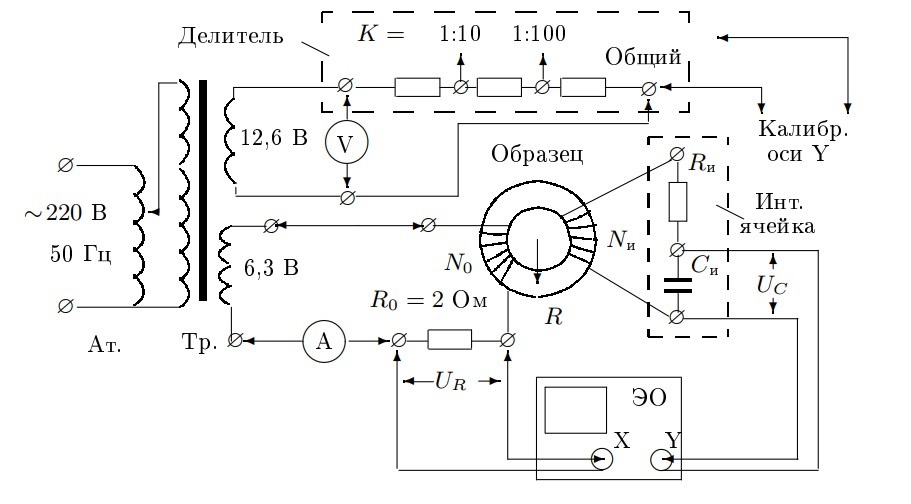
\includegraphics[width=140mm]{scheme.png}
\caption{Схема установки для изучения петли гистерезиса и калебровки приборов}\label{schema}
\end{figure}

В этой работе величины $K_x$ и $K_y$ указаны на Большое деление, в то время как все деления указаны в величинах маленьких делений, которые в 5 раз меньше больших.



\textbf{Параметры установки}:

$R_0 = 0.220 \pm 0.002 Ohm$
$R_u = 20kOhm$
$C_u = 20 \mu F$
\medskip

Феррит 1000

$N_0 = 42$ витка
$N_u = 400 $ витков
$S = 3,0 cm^2$
$2\pi R = 25 cm$
\medskip

Пермаллой

$N_0 = 20$ витка
$N_u = 300 $ витков
$S = 0,76 cm^2$
$2\pi R = 13,3 cm$
\medskip

Кремнистое железо

$N_0 = 25$ витка
$N_u = 250 $ витков
$S = 2,0 cm^2$
$2\pi R = 11 cm$


Формулы для расчёта цены деления осциллографа:
\begin{equation}
H = \frac{K_x N_0}{2\pi R R_0}*x;   B = \frac{K_yR_uC_u}{SN_u}*y   .
\end{equation}

\bigskip

\subsection*{Ход работы}
\bigskip

\subsubsection*{Калибровка}

\textbf{Ось Х:}

Коэффициент усиления рассчитывается по формуле:

\begin{equation}
m_x = \frac{2\sqrt{2} R_0 I_{eff}}{2x} \left[ \frac{V}{div} \right]
\end{equation}

где $I_{eff}$ - показания амперметра.

Для параметров:
$K_x = 50mV/div$;
$2x = [50 \pm 0.5]div$;
$I_{Eff} = [0,767 \pm 0,001]A$ 

Получено значение $\bm{m_x = [47.8\pm 0.8]mV/div}$, что показывает, что осциллограф даёт на самом деле усиление, на 4\% отличное от ожидаемого для оси Х.  (Ну или что где-то тут неточность)

\textbf{Ось У:}

Коэффициент усиления рассчитывается по формуле:

\begin{equation}
m_y = \frac{2\sqrt{2} U_{eff}}{2y} \left[ \frac{V}{div} \right]
\end{equation}

где $U_{eff}$ - показания вольтметра.

Для параметров:
$K_y = 20 mV/div$;
$2y = [41 \pm 0.5] div$;
$U_{eff} = [58,3 \pm 0,2] mV$

Получено значение $\bm{m_y = [20.1\pm 0.3]mV/div}$, что совпадает с нашими ожиданиями.

Для параметров:
$K_y  = 50 mV/div$;
$2y = [38 \pm 0.5] div$;
$U_{eff} = [135 \pm 1] mV$

Получено значение \boldmath$m_y = [50.2\pm 0.8]mV/div$\unboldmath, что совпадает с нашими ожиданиями.

\subsubsection*{Определение $\bm{\tau$}}

\begin{equation}
\tau = RC = \frac{U_\text{вх}}{\Omega U_\text{вых}}
\end{equation}

где $\Omega = 2\pi * 50Hz$ - частота тока в установке.
Данные:

Вход:
$K_y = 1V$
$2y_\text{вх} = [38 \pm 0.5] div$; 
Выход:

$K_y = 10mV$
$2y_\text{вых} = [30 \pm 0.5] div$.

Откуда получаем: $\bm{\tau = [403 \pm 9]msec}$, что идеально совпадает с расчётом $\tau$ через параметры установки: $\bm{\tau = C_uR_u = [400 \pm 4]msec}$.

\subsubsection*{Исследование гистерезиса}

\begin{figure}[ht]
\centering
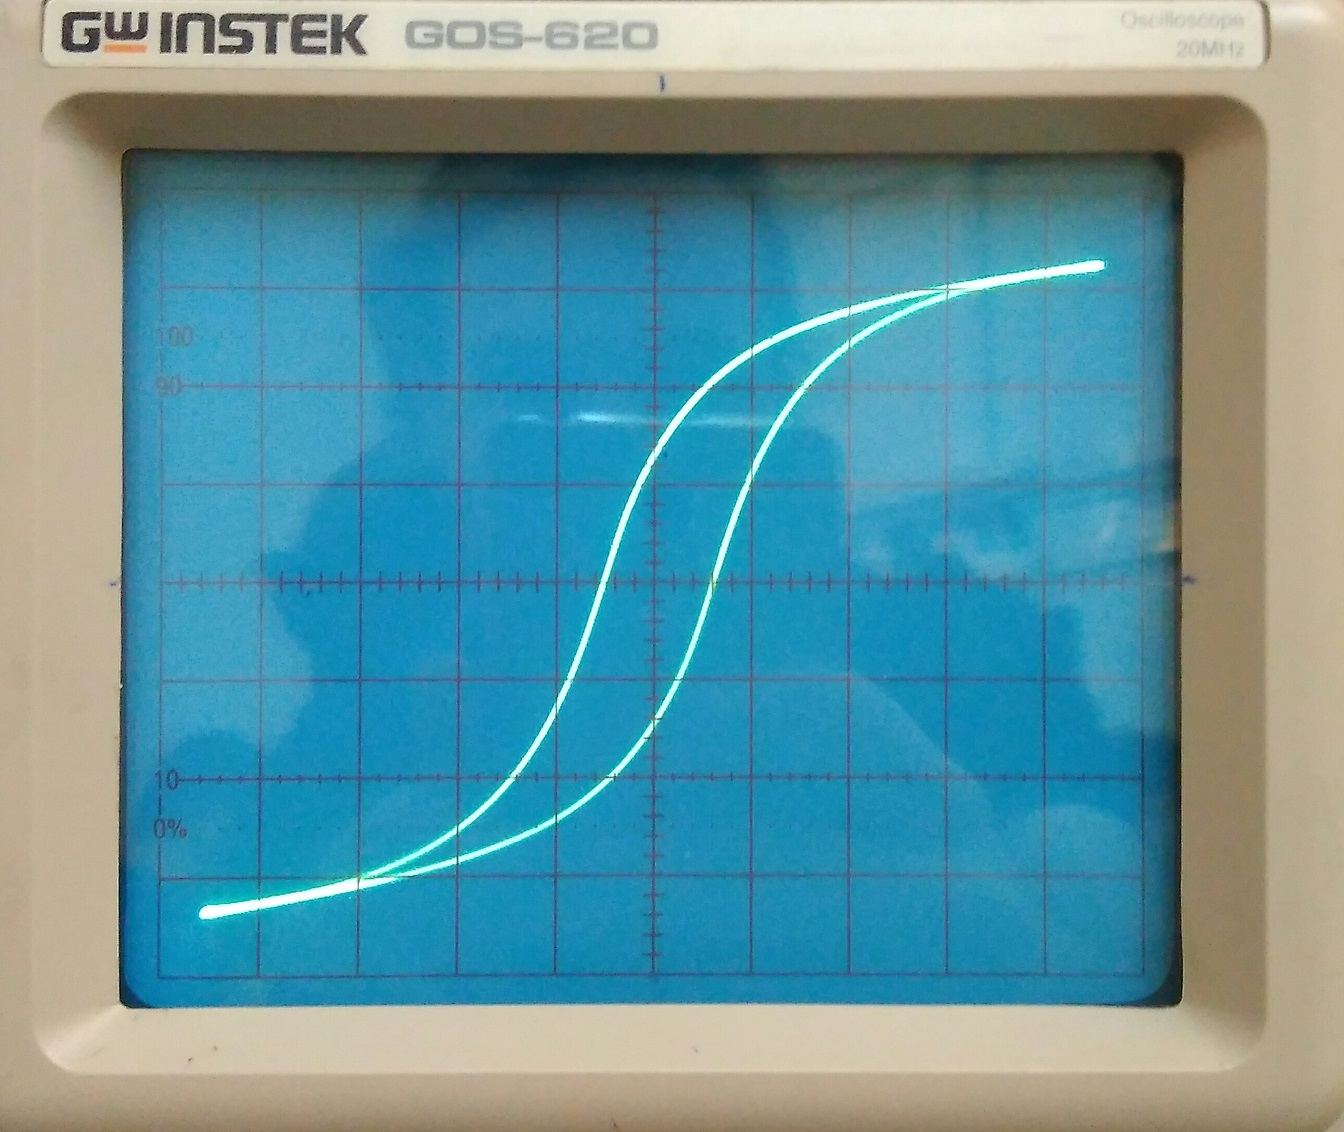
\includegraphics[width=55mm]{Ferrit.jpg} 
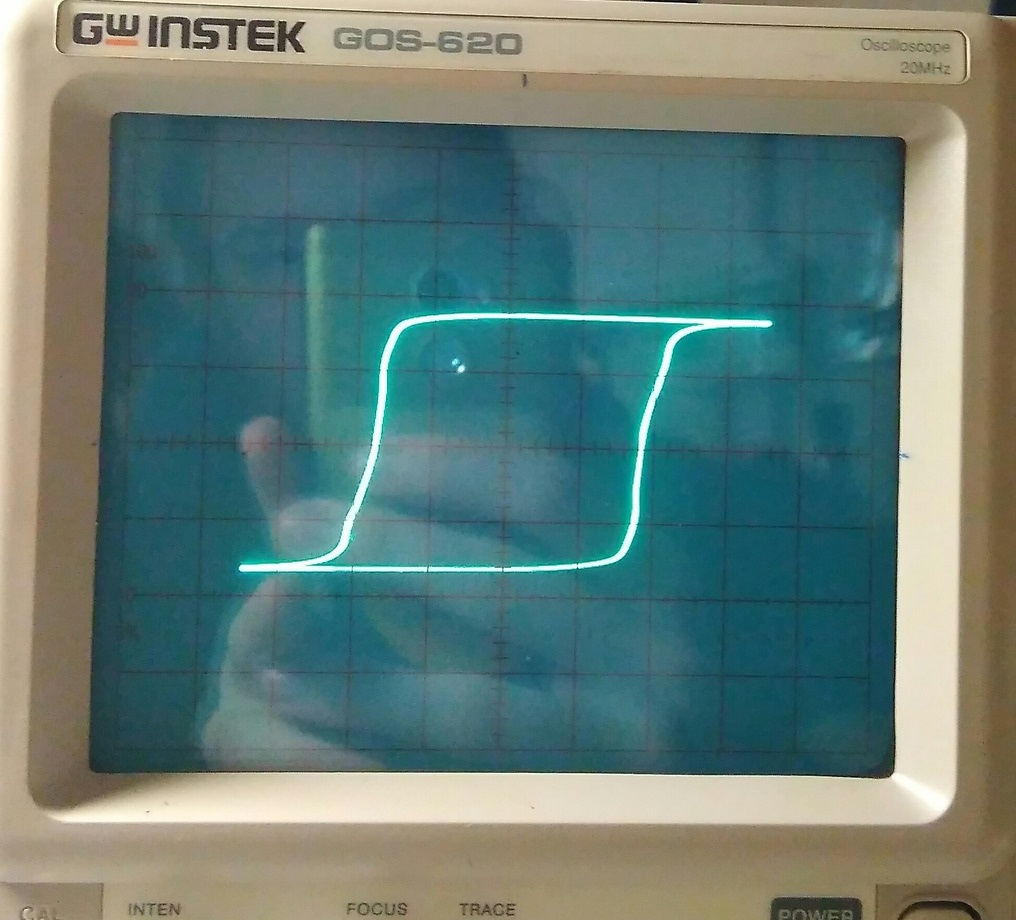
\includegraphics[width=55mm]{Perm.jpg}
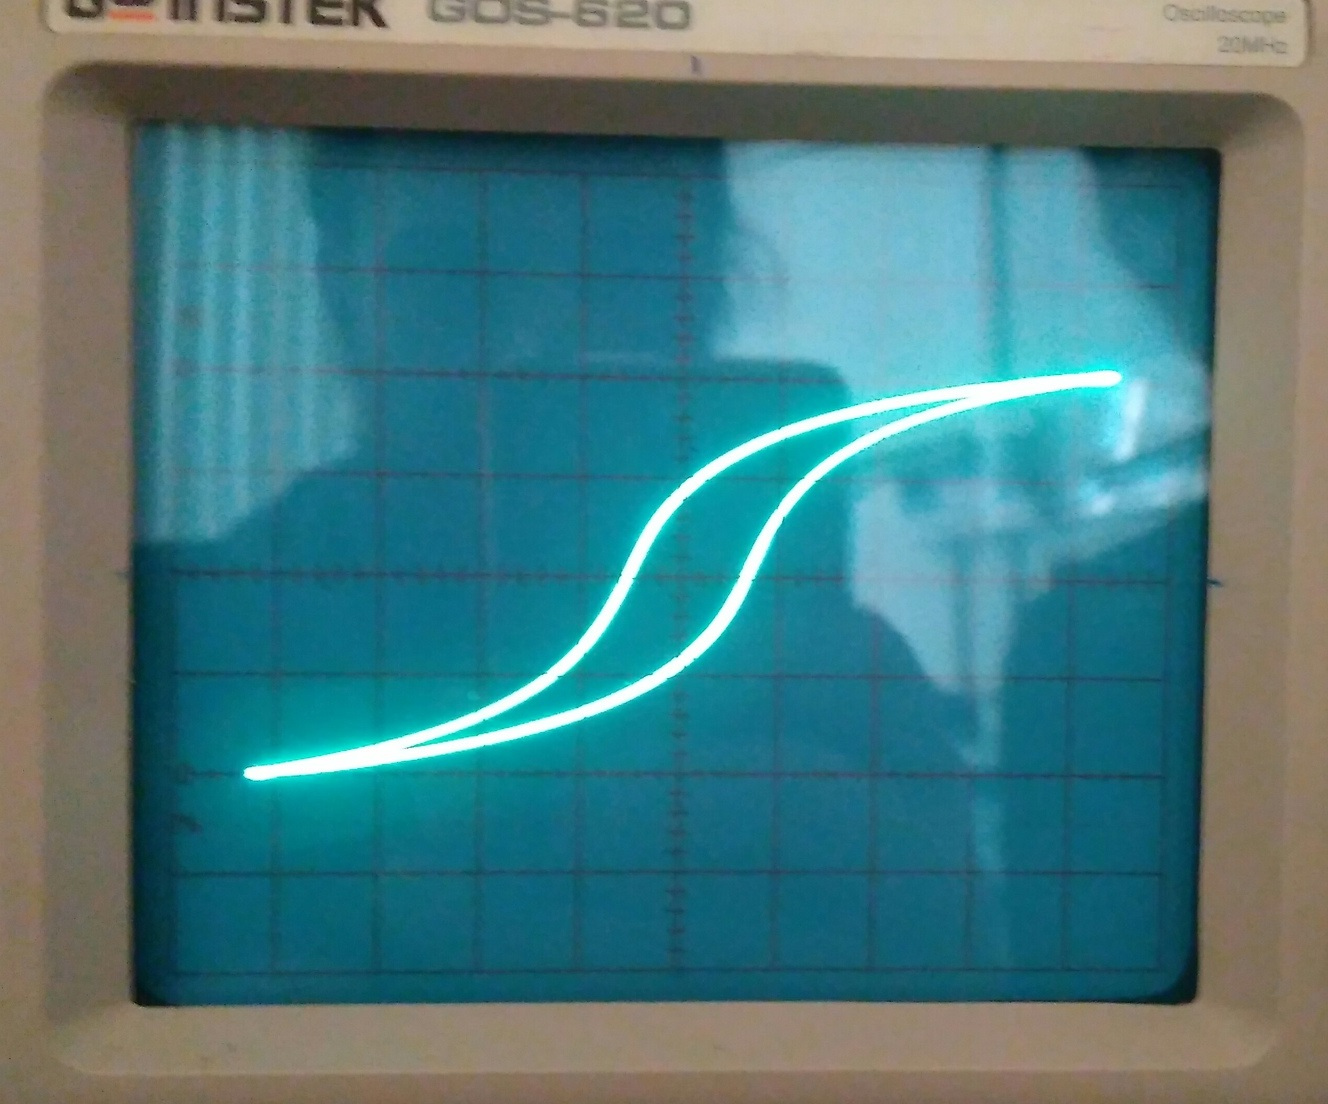
\includegraphics[width=55mm]{Kremn_Ferr.jpg}
\caption{Петля гистерезиса для образцов из феррита (слева), пермаллоя (по центру) и кремниестого железа (справа)}\label{schema}
\end{figure}

\begin{figure}[ht]
\centering
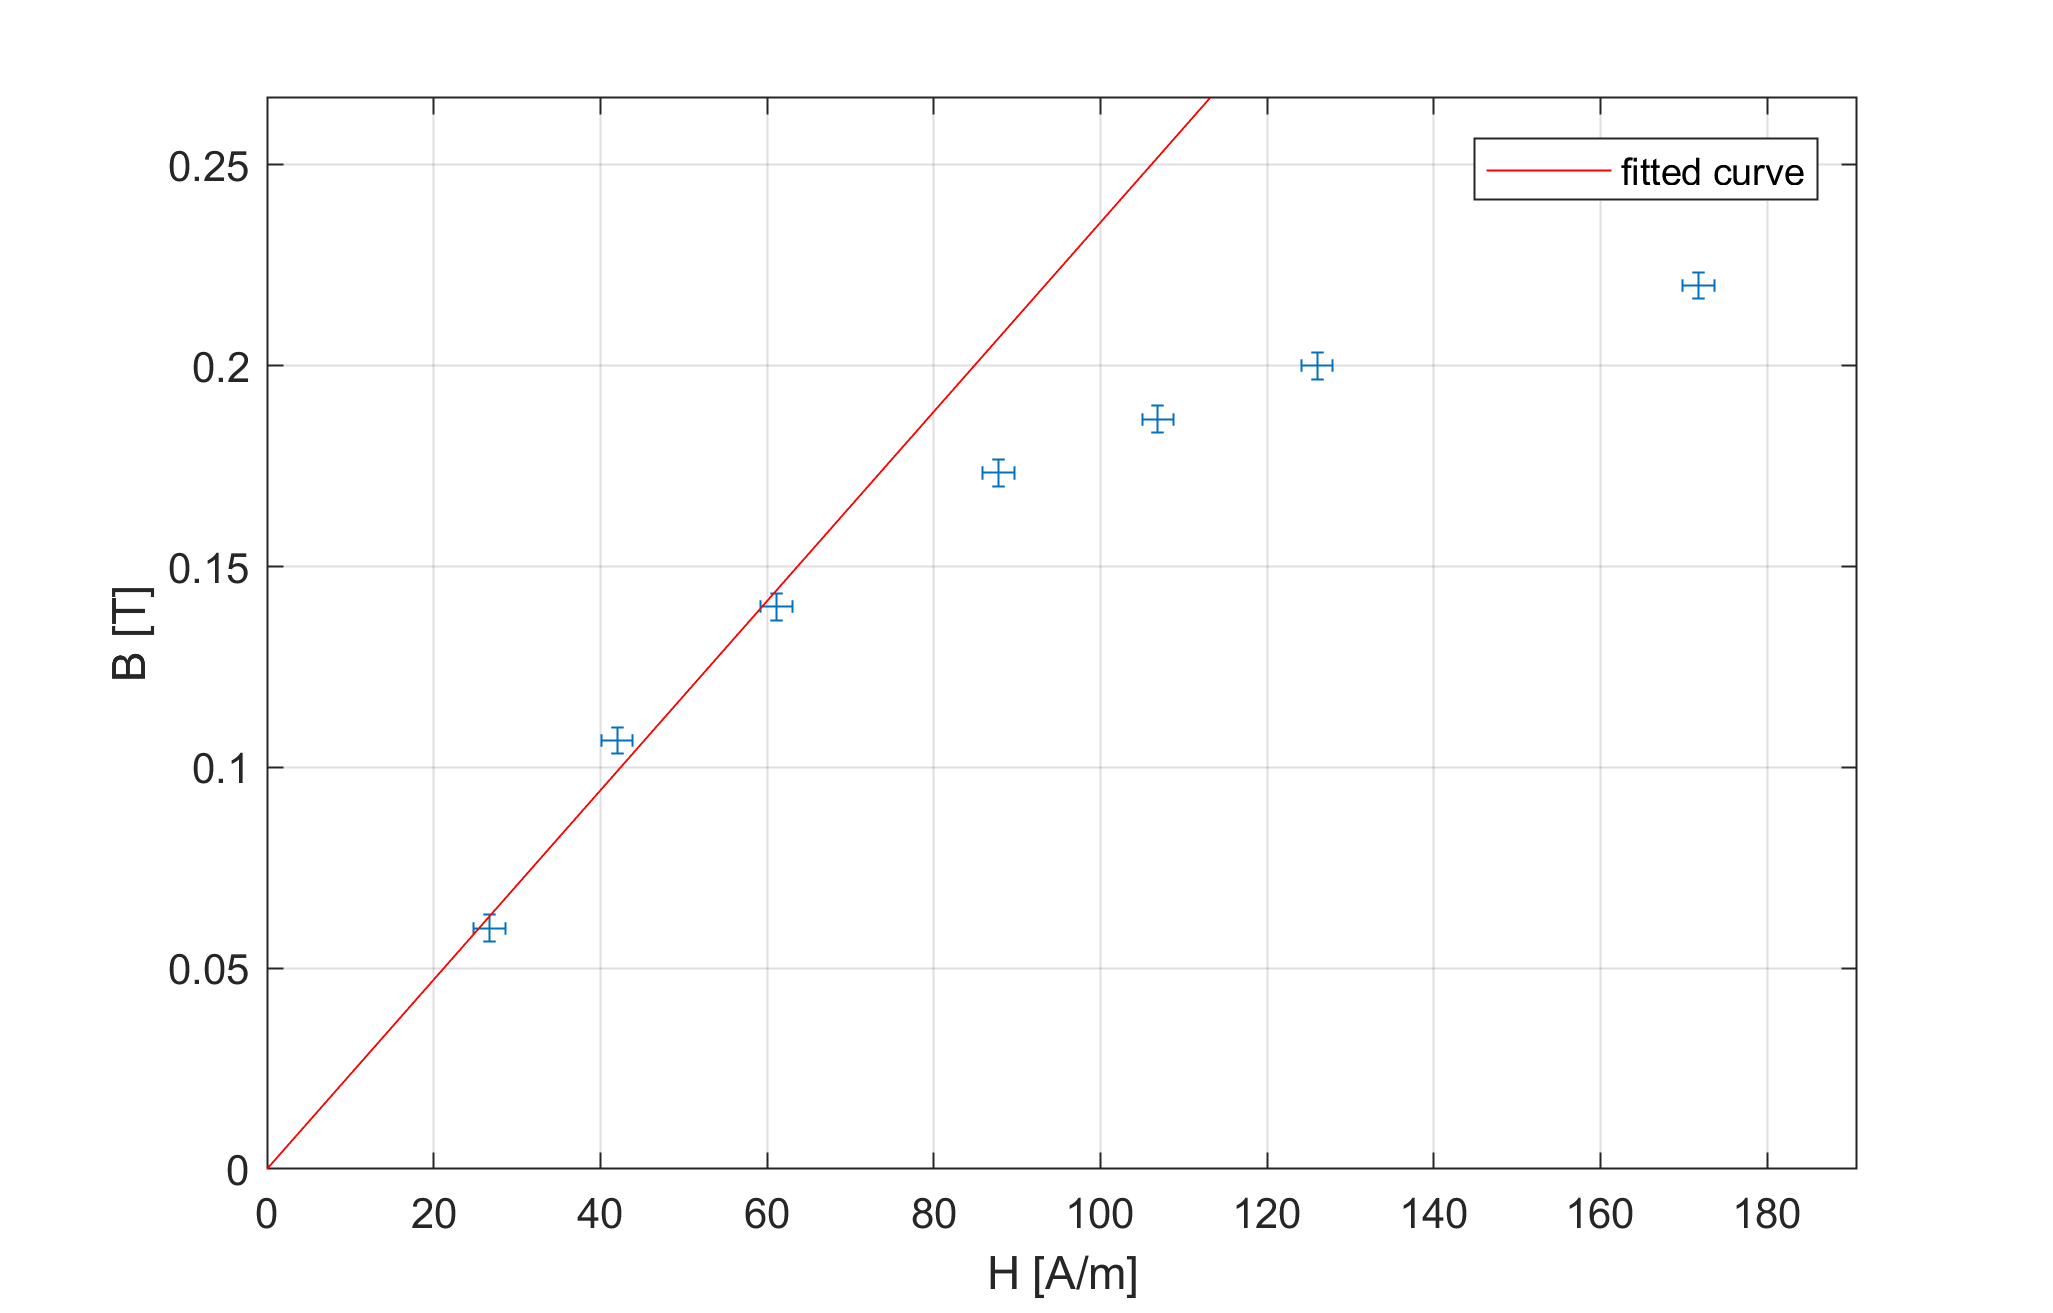
\includegraphics[width=110mm]{PlotFerrit.png}
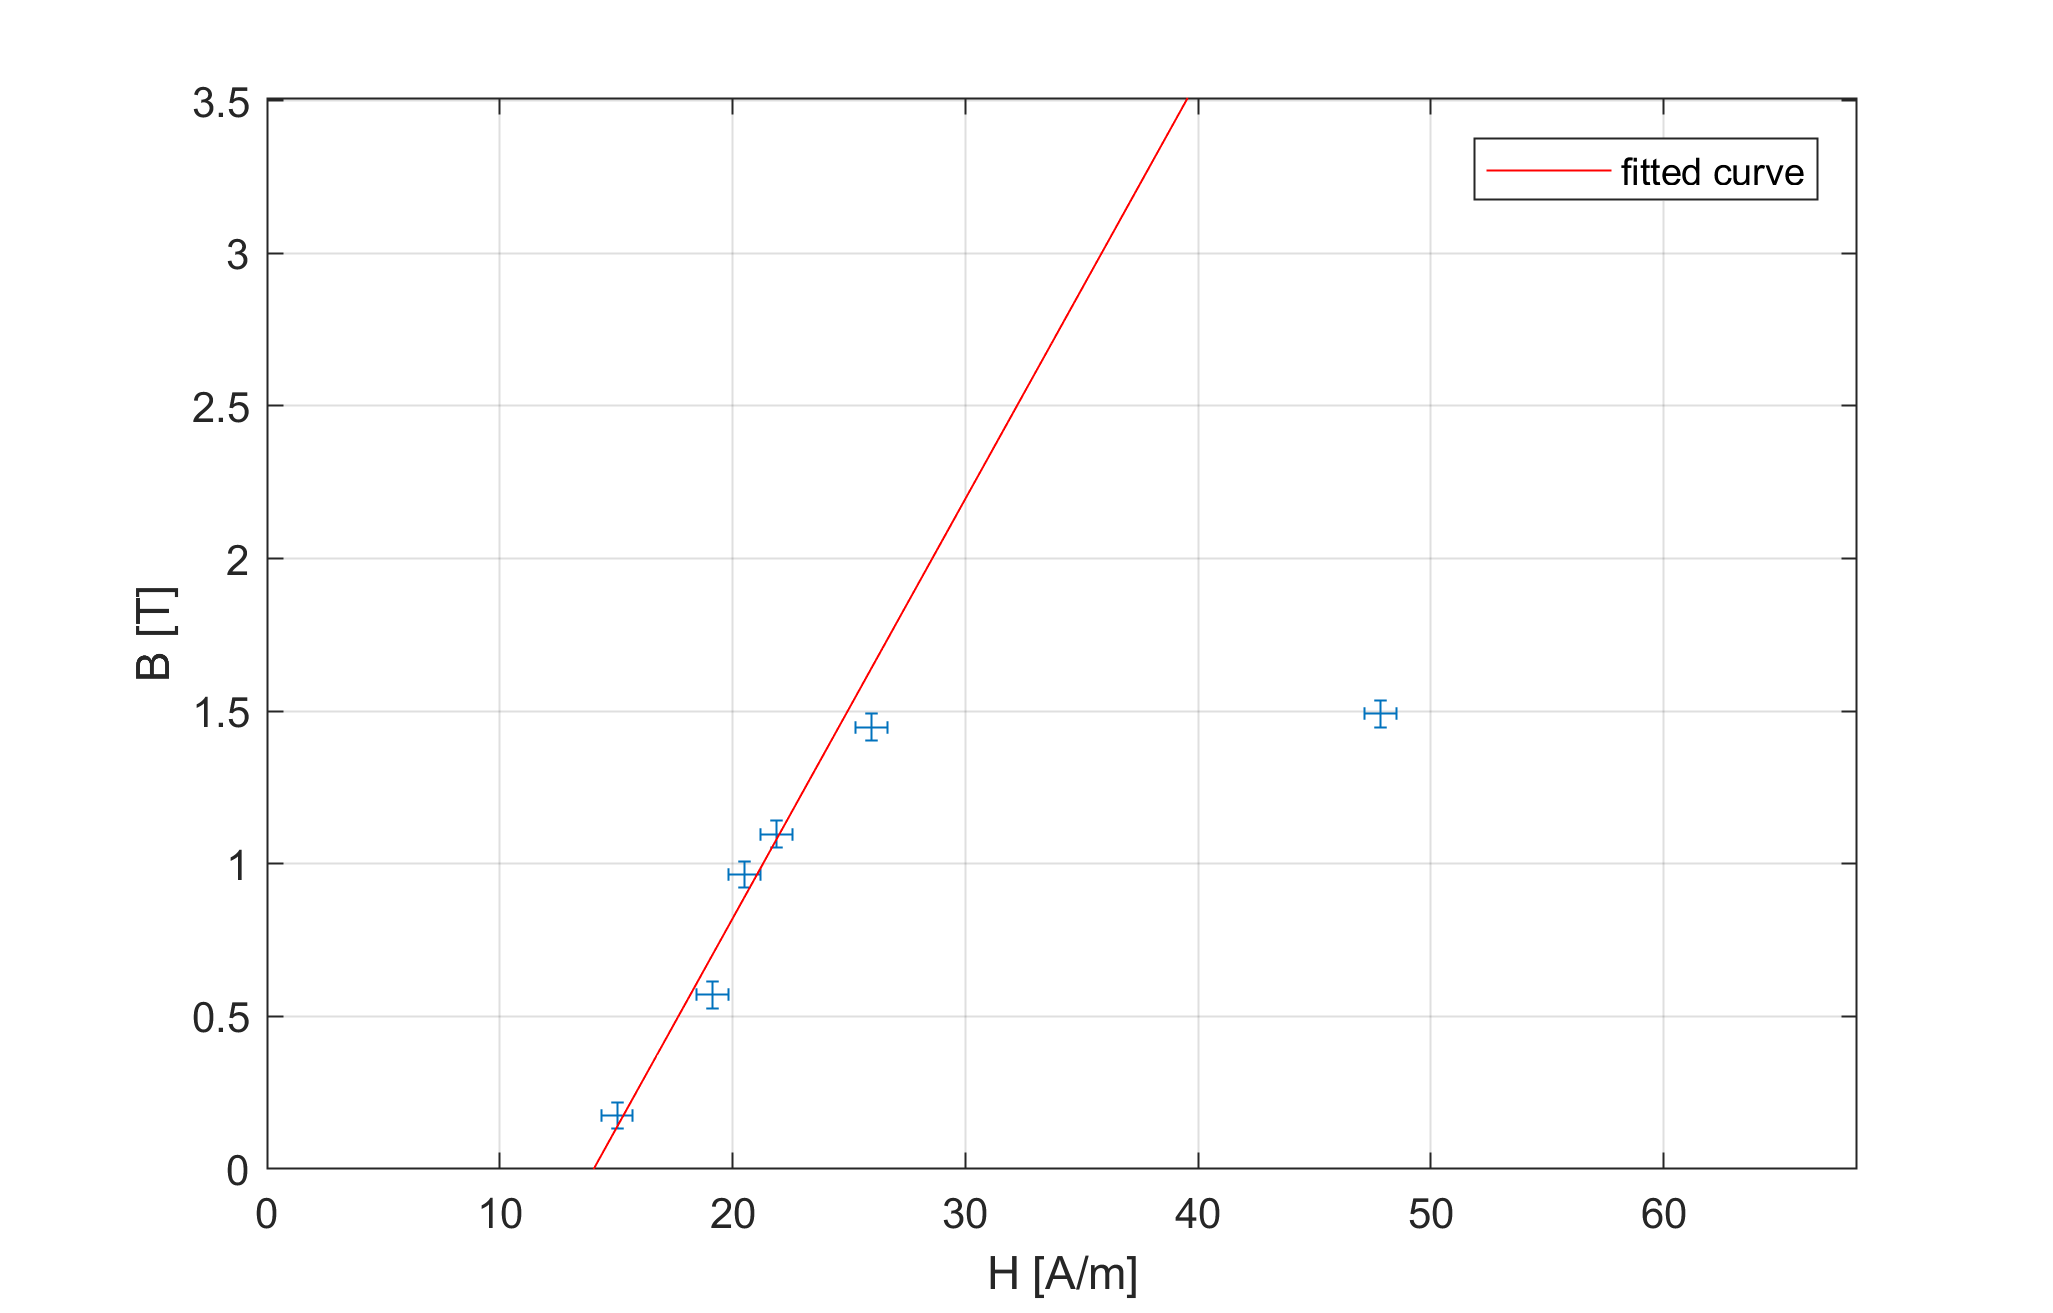
\includegraphics[width=110mm]{PlotPermalloy.png}
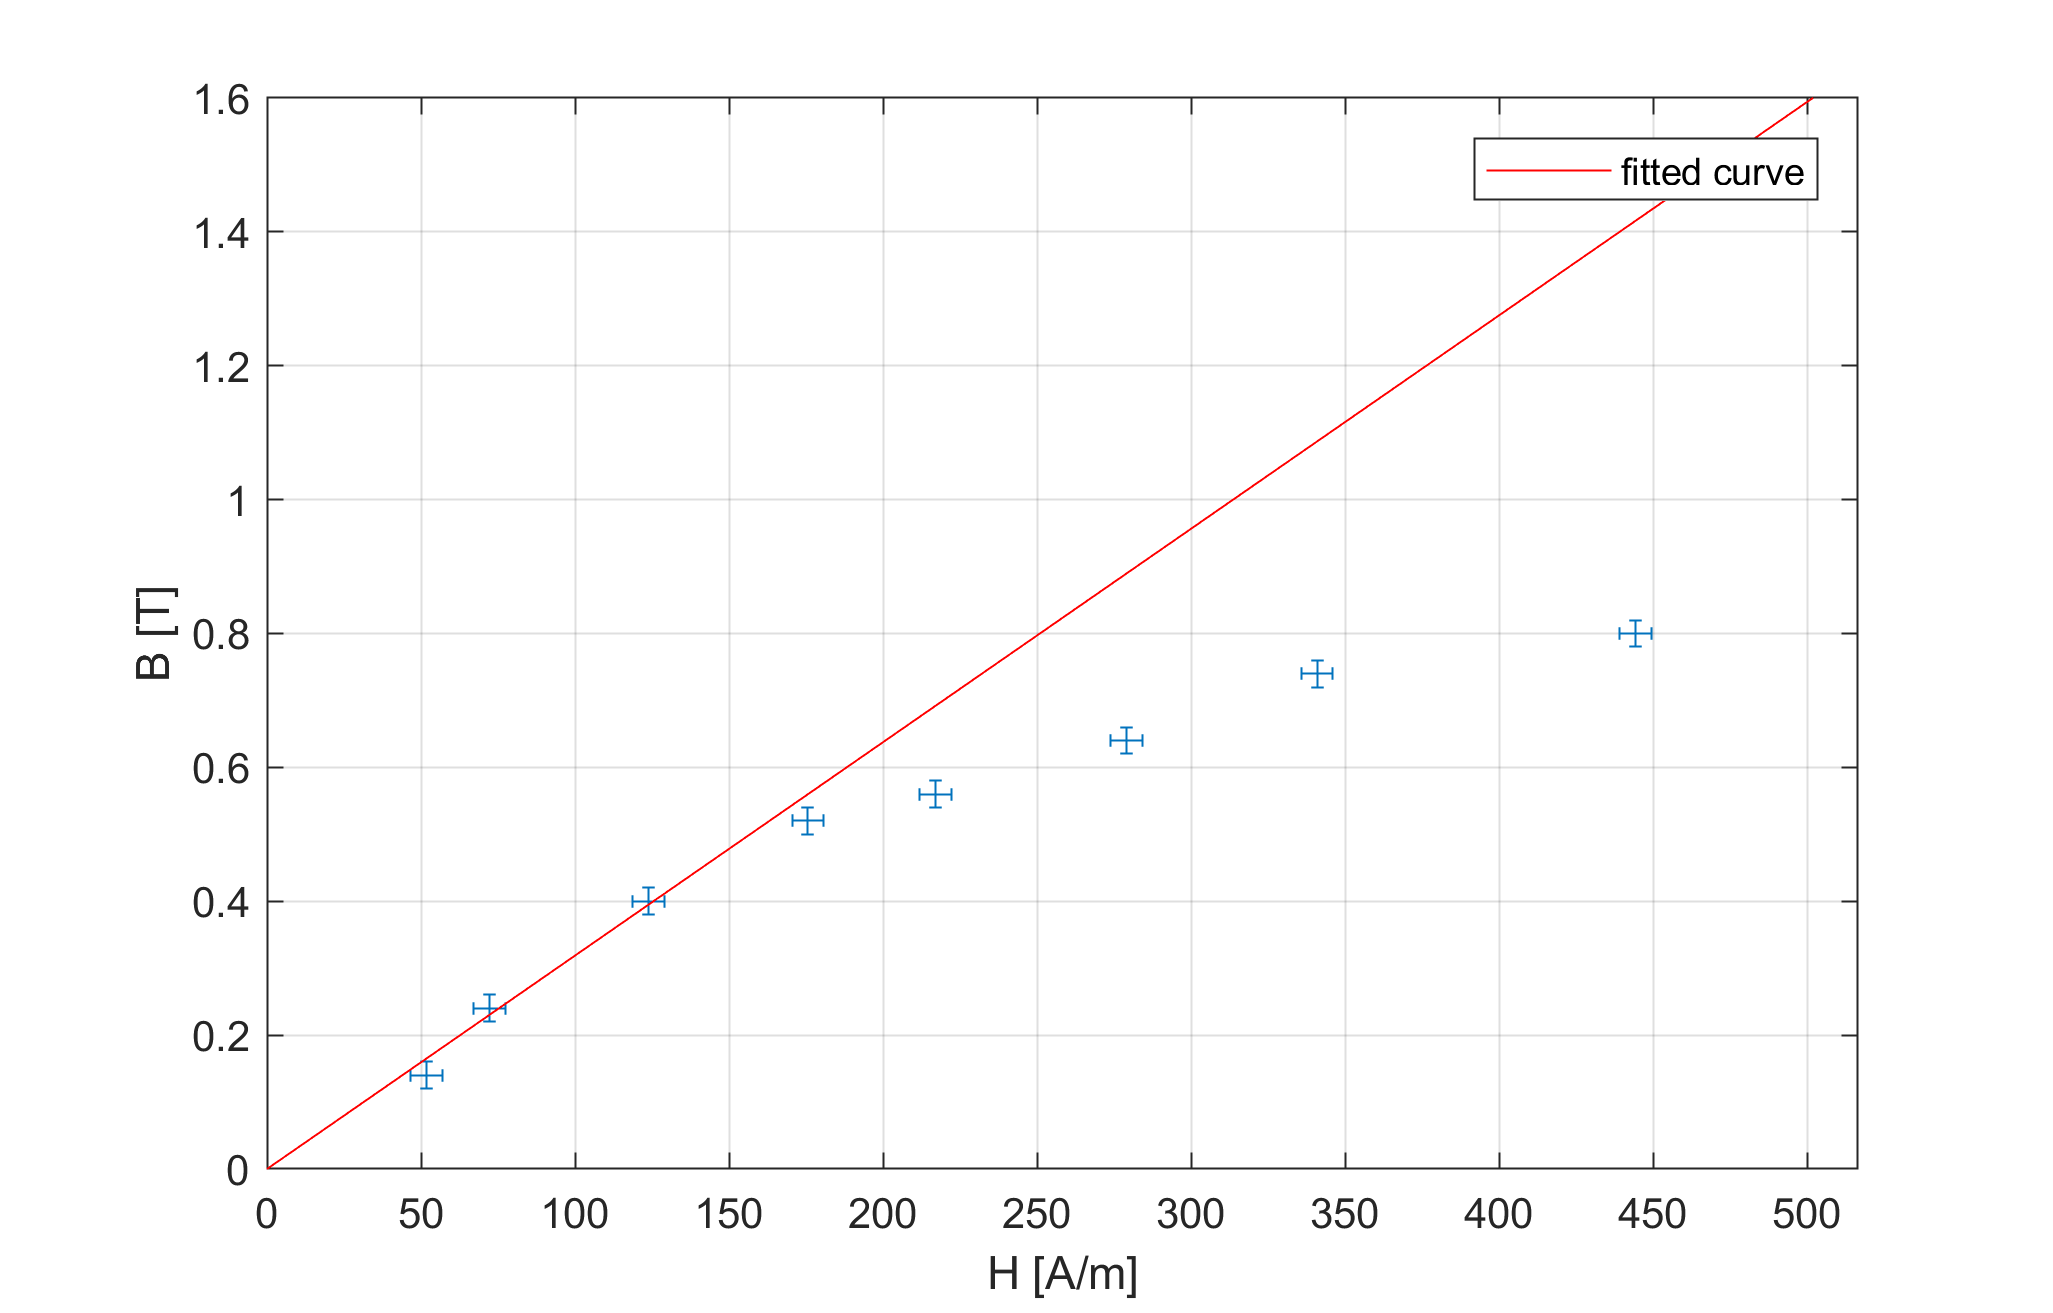
\includegraphics[width=110mm]{PlotKrem_Ferr.png}
\caption{Кривые намагничивания для образцов из феррита (сверху), пермаллоя (по центру) и кремниестого железа (снизу)}\label{graphs}
\end{figure}



\subparagraph{Полученные результаты:}

Полученные кривые намагничивания можно видеть на графиках \ref{graphs}.

Полученные значения для коэрцитивной силы $H_c$, индукции насыщения $B_s$ и коэффициента намагничивания $\mu_\text{диф}$:

Феррит: \hfill$H_c = [23.3 \pm 1.1]A/m$; $B_s = [0.240 \pm 0.006]T$; $\mu_\text{диф} = [2.4 \pm 0.2]mT*m/A$

Пермаллой: \hfill$H_c = [24.9 \pm 1.1]A/m$; $B_s = [1.49 \pm 0.05]T$; $\mu_\text{диф} = [140 \pm 30]mT*m/A$

Кремнистое железо: \hfill$H_c = [66 \pm 3]A/m$; $B_s = [0.88 \pm 0.03]T$; $\mu_\text{диф} = [3.2 \pm 0.3]mT*m/A$



\bigskip

\subsection*{Итог}
\bigskip

В данной работе мы пронаблюдали эффект гистерезиса в ферромагнетиках. 

Также были получены некоторые характеристики исследуемых веществ:
\medskip

\begin{tabular}{|c|c|c|c|}
\hline
Величина & Феррит & Пермаллой & Кремнистое железо \\ \hline
$H_c, A/m$ 			 & $23.3 \pm 1.1$  &  $24.9 \pm 1.1 $ & $66 \pm 3$  \\ \hline
$B_s, T$			 &$0.240 \pm 0.006$  &  $1.49 \pm 0.05 $ & $0.88 \pm 0.03 $     \\ \hline
$\mu_\text{диф}, mT*m/A$ &$2.4 \pm 0.2$ &   $140 \pm 30 $ & $3.2 \pm 0.3 $  \\ \hline
\end{tabular}

\medskip
Табличные же значения очень сильно зависят от пропорции элементов в сплаве. Примерные диапазоны приведены в табличке:
\medskip

\begin{tabular}{|c|c|c|c|}
\hline
Величина & Феррит & Пермаллой & Кремнистое железо \\ \hline
$H_c, A/m$ 			 & $\approx 10 $  &  $1 - 100 $ & $10 - 100$  \\ \hline
$B_s, T$			 &$\approx 0.25$  &  $1 - 2 $ & $1 - 2 $     \\ \hline
$\mu_\text{диф}, mT*m/A$ &$0.2 - 8$ &   $\approx 100$ & $\approx 10 $  \\ \hline
\end{tabular}
\bigskip

\subsection*{Приложение}
\bigskip
\subparagraph{Исходные данные:}

2) - параметры для петли гистерезиса, что на картинке

3) - параметры для кривой намагничивания

4) - данные для определения коэрцитивной силы $H_c$ и индукции насыщения $B_s$

\medskip

Феррит 

2)
$K_x = 50mV/div$;
$K_y = 20mV/div$;
$I_{eff} = 0.6454 \pm 0.0002 A$

3)Кривая снята при тех же $K_x; K_y$

4)
$2y = 36 div$
($K_y = 20mV/div$);
$2x = 30.5 div$
($K_x = 10 mV/div$)
\medskip

Пермаллой:

2)
$K_x = 20mV/div$;
$K_y = 50mV/div$;
$I_{eff} = 0.173 \pm 0.001 A$

3)Кривая снята при тех же $K_x; K_y$

4)
$2y = 17 div$
($K_y = 50mV/div$);
$2x = 36,5 div$
($K_x = 10 mV/div$)
\medskip

Кремнистое железо:

2)
$K_x = 0.1V/div$;
$K_y = 50mV/div$;
$I_{eff} = 1.252 \pm 0.002 A$

3)Кривая снята при тех же $K_x; K_y$

4)
$2y = 22 div$
($K_y = 50mV/div$);
$2x = 32 div$
($K_x = 20 mV/div$)
\end{document} % конец документа